%
%
%

\begin{frame}[t,allowframebreaks]{Applying a nonlinear model to the XOR problem -} 

    To solve the problem, we can try a {\bf deeper architecture}.
    \begin{itemize}
        \item 
        For example, we can consider a simple feedforward network 
        with a single hidden layer.\\
    \end{itemize}
    \vspace{0.2cm}

    {\bf What types of functions would be computed} at each layer?\\
    \begin{itemize}
    \item
        {\bf Linear functions have desirable properties}.
    \item
        However, they {\bf they cannot all be linear!}    
        \begin{itemize}
            \item 
            If they were, in spite of its greater depth, 
            the network as a whole would remain a linear function of $\mathbf{x}$
            (and linear models cannot learn XOR).
            % \item 
            % We have just seen that linear models cannot learn the XOR function!
        \end{itemize}
    \end{itemize}
    \vspace{0.2cm}

    We can still use a {\bf linear regression model at the output}.\\
    \vspace{0.2cm}

    However, the {\bf linear model would be applied to transformed features} 
    generated by non-linear functions at the hidden layer.\\
    \vspace{0.2cm}

    In essence, we are {\bf aiming to learn a new representation of the inputs}
    that is linearly separable!\\

    \framebreak

    In essence, we are {\bf aiming to learn a new representation of the inputs}
    that is linearly separable!
    {\bf Representation learning} is a central idea in \gls{dl}.\\

    \begin{center}
        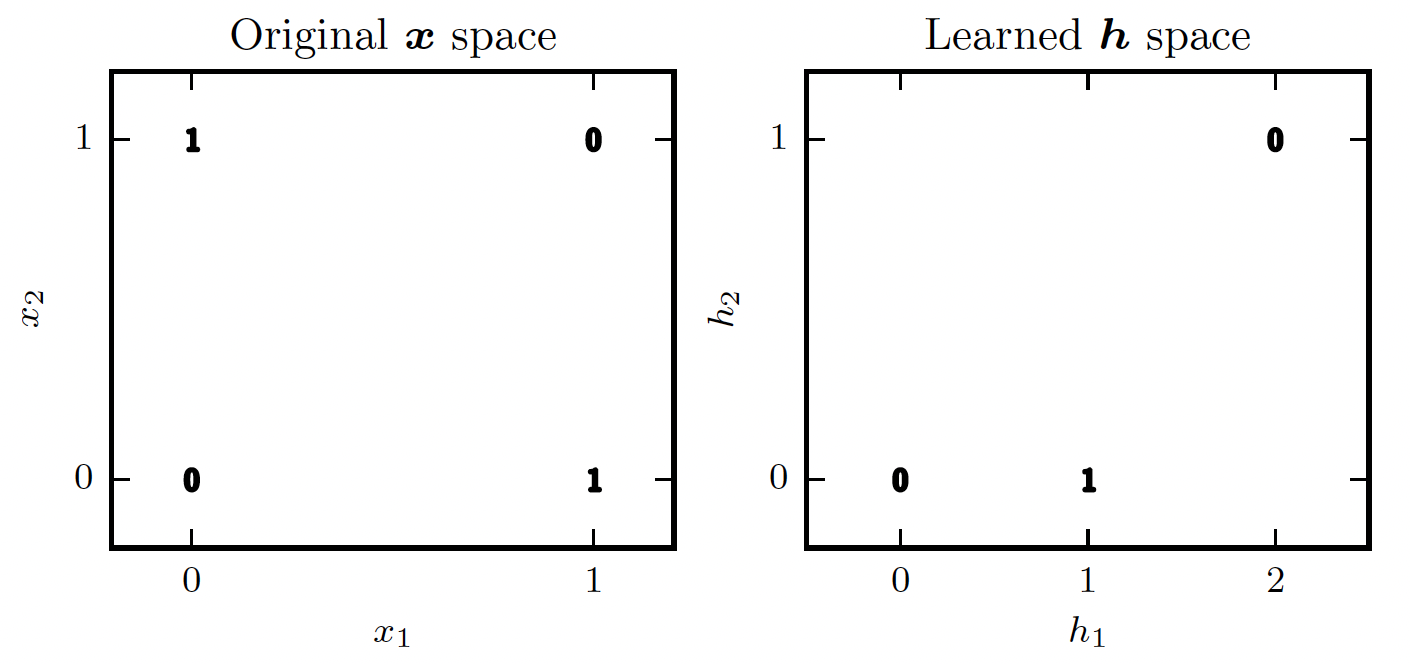
\includegraphics[width=0.90\textwidth]
        {./images/xor/goodfellow17_xor_learned_representations_01.png}\\
     {\scriptsize 
      Solving the XOR problem by learning a representation.\\
      \color{col:attribution} 
      Image reproduced from p. 168 of \cite{Goodfellow:2017MITDL} (Fig. 6.1)}\\
    \end{center}

    \framebreak

    A diagram of our feedforward network is given below.\\
    \begin{center}
        \begin{tikzpicture}[scale=0.98]
          %\draw[help lines] (0,0) grid (8,6);
          \node[ann_processing_node] (o)  at (7.0, 2.5) {$\hat{y}$};
      
          \node[ann_processing_node] (h1) at (4.0, 3.5) {$h_1$};
          \node[ann_processing_node] (h2) at (4.0, 1.5) {$h_2$};
          \node[ann_bias_node]       (b)  at (5.0, 0.0) {$+1$};
      
          \node[ann_input_node]      (x1) at (0.0, 3.5) {$x_1$};
          \node[ann_input_node]      (x2) at (0.0, 1.5) {$x_2$};
          \node[ann_bias_node]       (c1) at (1.0, 5.0) {$+1$};
          \node[ann_bias_node]       (c2) at (1.0, 0.0) {$+1$};
      
          % from input layer to h1
          \drawgraphlinebigarrow (x1.east) 
          to node[above, midway] 
          {\scriptsize $W_{11}$}(h1.west) ;
      
          \drawgraphlinebigarrow (x2.east) 
          to node[below, midway] 
          {\scriptsize $W_{21}$}(h1.south west) ;
      
          \drawgraphlinebigarrow (c1.east) 
          to node[above, midway] 
          {\scriptsize $c_1$}(h1.north west) ;
      
          % from input layer to h2
          \drawgraphlinebigarrow (x1.east) 
          to node[above, midway] 
          {\scriptsize $W_{12}$}(h2.north west) ;
      
          \drawgraphlinebigarrow (x2.east) 
          to node[below, midway] 
          {\scriptsize $W_{22}$}(h2.west) ;
      
          \drawgraphlinebigarrow (c2.east) 
          to node[below, midway] 
          {\scriptsize $c_2$}(h2.south west) ;
      
          % from hidden layer to output
          \drawgraphlinebigarrow (h1.east) 
          to node[above, midway] 
          {\scriptsize $w_1$}(o.north west) ;
      
          \drawgraphlinebigarrow (h2.east) 
          to node[above, midway] 
          {\scriptsize $w_2$}(o.south west) ;
      
          \drawgraphlinebigarrow (b.east) 
          to node[below, midway] 
          {\scriptsize $b$}(o.south) ;
      
          % \drawgraphlinebigarrow (o.east) 
          % to node[above,midway] 
          % {\scriptsize \color{black} $f(\mathbf{h};\mathbf{w},b)$} (10.0,2.5);
      
        \end{tikzpicture}
    \end{center}        

    \framebreak

    The output node computes the function 
    $f^{(1)}: \mathbb{R}^2 \rightarrow \mathbb{R}$
    \begin{equation}
        \hat{y} = 
        f^{(1)}(\mathbf{h};\mathbf{w},b)
        \label{eq:learn_xor_nonlinear_model_f1}
    \end{equation}        
    whereas the hidden layer nodes
    compute the function
    $f^{(2)}: \mathbb{R}^2 \rightarrow \mathbb{R}^2$
    \begin{equation}
        \mathbf{h} = 
        f^{(2)}(\mathbf{x};\mathbf{W},\mathbf{c})
        \label{eq:learn_xor_nonlinear_model_f2}
    \end{equation}        
    The network computes the composite function 
    $f^{(1)} \circ f^{(2)}: \mathbb{R}^2 \rightarrow \mathbb{R}$
    \begin{equation}
        \hat{y} = 
        f^{(1)}\Big(f^{(2)}(\mathbf{x};\mathbf{W},\mathbf{c});\mathbf{w},b\Big)
        \label{eq:learn_xor_nonlinear_model_f1f2}
    \end{equation}        
      
    \framebreak

    The output is still a {\bf linear regression model} 
    applied to features $\mathbf{h}$:\\
    \begin{equation}
        \hat{y} = 
        f^{(1)}(\mathbf{h};\mathbf{w},b) = 
        \begin{pmatrix}
            w_1 & w_2 \\
        \end{pmatrix} 
        \cdot
        \begin{pmatrix}
            h_1 \\ 
            h_2 \\
        \end{pmatrix} 
        + b =
        \mathbf{w}^{T} \mathbf{h} + b 
        \label{eq:learn_xor_nonlinear_model_out}
    \end{equation}

    The features $\mathbf{h}$ are computed by transforming a linear combination 
    of the network inputs $\mathbf{x}$ with a non-linear activation function $g$:
    \begin{equation}
        \mathbf{h} = 
        f^{(2)}(\mathbf{x};\mathbf{W},\mathbf{c}) = 
        g\Bigg\{
            \begin{pmatrix}
                W_{11} & W_{21} \\
                W_{12} & W_{22} \\
            \end{pmatrix} 
            \cdot
            \begin{pmatrix}
                x_1 \\ 
                x_2 \\
            \end{pmatrix} 
            + 
            \begin{pmatrix}
                c_1 \\ 
                c_2 \\
            \end{pmatrix}
        \Bigg\} =
        g(\mathbf{W}^{T} \mathbf{x} + \mathbf{c})
        \label{eq:learn_xor_nonlinear_model_activation}
    \end{equation}

    The activation function $g$ is {\bf applied element-wise}.\\ 
    \vspace{0.2cm}
    There are several choices of activation functions, 
    but in modern networks the standard choice is the 
    {\bf piecewise linear} \gls{relu} function:
    \begin{equation}
        g(z) = max(0.,z)
        \label{eq:learn_xor_nonlinear_model_activation_relu}
    \end{equation}

    \framebreak

    From Eqs.~
    \ref{eq:learn_xor_nonlinear_model_f1}-\ref{eq:learn_xor_nonlinear_model_activation_relu},
    the composite function computed by the network
    can be written as:
    \begin{equation}
        \hat{y} = 
        f^{(1)}\Big(f^{(2)}(\mathbf{x};\mathbf{W},\mathbf{c});\mathbf{w},b\Big) =
        \mathbf{w}^{T} max(0, \mathbf{W}^{T} \mathbf{x} + \mathbf{c}) + b 
        \label{eq:learn_xor_nonlinear_model_final}
    \end{equation}        

    The weights $\mathbf{W}$, $\mathbf{w}$, and biases $\mathbf{c}$, and $b$
    that provide a solution to the problem of learning the XOR function, are 
    given in \cite{Goodfellow:2017MITDL}:
    \begin{equation}    
        \mathbf{W} = 
        \begin{pmatrix}
            1 & 1 \\
            1 & 1 \\
        \end{pmatrix}, 
        \;\; 
        \mathbf{w} = 
        \begin{pmatrix}
            1  \\
            -2 \\
        \end{pmatrix}, 
        \;\;
        \mathbf{c} = 
        \begin{pmatrix}
            0 \\
            -1 \\
        \end{pmatrix},         
        \;\;         
        and \;\; b = 0
        \label{eq:learn_xor_nonlinear_model_weights}
    \end{equation}

    Substituting Eq.~\ref{eq:learn_xor_nonlinear_model_weights} in 
    Eq.~\ref{eq:learn_xor_nonlinear_model_activation}, we obtain:
    \begin{equation}
        \mathbf{h} = 
        \begin{pmatrix}
            h_1 \\ 
            h_2 \\
        \end{pmatrix} =
        max \Bigg\{0, 
        \begin{pmatrix}
            1 & 1 \\
            1 & 1 \\
        \end{pmatrix} 
        \cdot
        \begin{pmatrix}
            x_1 \\
            x_2 \\
        \end{pmatrix}
        +         
        \begin{pmatrix}
            0 \\
            -1 \\
        \end{pmatrix}
        \Bigg\} =
        max \Bigg\{0, 
        \begin{pmatrix}
          x_1+x_2     \\ 
          x_1+x_2-1   \\
        \end{pmatrix}
        \Bigg\}
        \label{eq:learn_xor_nonlinear_model_h} 
    \end{equation}

    \framebreak

    Further substitution of 
    Eq.~\ref{eq:learn_xor_nonlinear_model_weights} and
    Eq.~\ref{eq:learn_xor_nonlinear_model_h} in
    Eq.~\ref{eq:learn_xor_nonlinear_model_final}, yields:
    \begin{equation*}
        \hat{y} = 
        \begin{pmatrix}
            1  & -2 \\
        \end{pmatrix} 
        \cdot
        max \Bigg\{0, 
        \begin{pmatrix}
          x_1+x_2     \\ 
          x_1+x_2-1   \\
        \end{pmatrix}
        \Bigg\} \Rightarrow
    \end{equation*}        

    \begin{equation}
        \hat{y} = 
        max(0,x_1+x_2) - 2 max(0,x_1+x_2-1) =
        h_1 - 2 h_2
        \label{eq:learn_xor_nonlinear_model_final_w_weights}
    \end{equation}        

    It is worth recalling that the \gls{relu} function is applied element-wise.\\
    \vspace{0.2cm}

    \begin{columns}[t]
        \begin{column}{0.70\textwidth}
            \vspace{-1.1cm}
            \begin{center}
                \begin{tabular}{ c c | c || c  c | c }
                 $x_1$ & 
                 $x_2$ & 
                 {\bf \color{cadmiumred}$y$} & 
                 $h_1$     & 
                 $h_2$ & 
                 {\bf \color{cadmiumgreen}$\hat{y}$} \\ 
                 \hline
                  & 
                  & 
                 {\bf \color{cadmiumred}$x_1 \oplus x_2$} & 
                 $max(0,x_1+x_2)$     & 
                 $max(0,x_1+x_2-1)$ & 
                 {\bf \color{cadmiumgreen}$h_1-2h_2$} \\ 
                 \hline
                 0 & 0 & {\bf \color{cadmiumred}0} & 0 & 0 & {\bf \color{cadmiumgreen}0} \\  
                 0 & 1 & {\bf \color{cadmiumred}1} & 1 & 0 & {\bf \color{cadmiumgreen}1} \\   
                 1 & 0 & {\bf \color{cadmiumred}1} & 1 & 0 & {\bf \color{cadmiumgreen}1} \\  
                 1 & 1 & {\bf \color{cadmiumred}0} & 2 & 1 & {\bf \color{cadmiumgreen}0} \\   
                \end{tabular}
            \end{center}
        \end{column}
        \begin{column}{0.30\textwidth}
        \end{column}
    \end{columns}

\end{frame}


